\documentclass{article}

% If you're new to LaTeX, here's some short tutorials:
% https://www.overleaf.com/learn/latex/Learn_LaTeX_in_30_minutes
% https://en.wikibooks.org/wiki/LaTeX/Basics

% Formatting
\usepackage[utf8]{inputenc}
\usepackage[margin=1in]{geometry}
\usepackage[titletoc,title]{appendix}

% Math
% https://www.overleaf.com/learn/latex/Mathematical_expressions
% https://en.wikibooks.org/wiki/LaTeX/Mathematics
\usepackage{amsmath,amsfonts,amssymb,mathtools}

% Images
% https://www.overleaf.com/learn/latex/Inserting_Images
% https://en.wikibooks.org/wiki/LaTeX/Floats,_Figures_and_Captions
\usepackage{graphicx,float}
\usepackage{caption}
\usepackage{subcaption}

% Tables
% https://www.overleaf.com/learn/latex/Tables
% https://en.wikibooks.org/wiki/LaTeX/Tables

% Algorithms
% https://www.overleaf.com/learn/latex/algorithms
% https://en.wikibooks.org/wiki/LaTeX/Algorithms
\usepackage[ruled,vlined]{algorithm2e}
\usepackage{algorithmic}

% Code syntax highlighting
% https://www.overleaf.com/learn/latex/Code_Highlighting_with_minted
\usepackage{minted}
\usemintedstyle{borland}
\usepackage{listings}


% References
% https://www.overleaf.com/learn/latex/Bibliography_management_in_LaTeX
% https://en.wikibooks.org/wiki/LaTeX/Bibliography_Management
\usepackage{biblatex}
\addbibresource{references.bib}

% Title content
\title{AMATH 482 Homework 3}
\author{Rishabh Verma}
\date{February 24th, 2021}

\begin{document}

\maketitle

\begin{abstract}
    An object undergoing simple harmonic motion is filmed by three cameras in subpar lab conditions. The method of principal component analysis is used to isolate the simple harmonic motion from other factors, particularly noise and independent movement in extraneous dimensions. Principal component analysis is found to be an effective technique to identify patterns of variance in multi-dimensional data and isolate the most interesting feature.
\end{abstract}

\section{Introduction and Overview}
Consider a simple harmonic oscillator formed by a mass fixed to a spring. Under ideal circumstances, subjecting the mass to a non-zero initial velocity or non-zero initial displacement will cause the mass-spring system to undergo simple harmonic motion along the dimension given by the spring's orientation.

We can capture video data of the oscillator to study it, presenting the task of analyzing 1-D motion from 2-D videos in 3-D space. Sources of error may include:

\begin{itemize}
	\item The camera may be oriented in space such that the spring's dimension of motion does not perfectly match the camera's x-dimension or y-dimension.
	
	\item An imperfectly aligned initial setting causing extraneous motion along other dimensions. To make things more complicated, this dimension would be invisible to the camera if it is aligned with the camera's normal, suggesting the need for multiple cameras.
\end{itemize}

In order to develop a method to examine the ideal case, it is necessary to test this method and see how well it performs under extreme non-ideal conditions.

Data is captured from 4 experiments. In each experiment, an oscillating mass-spring system is videoed by three observers holding video cameras in radially different locations. Two of the observers hold their cameras vertically, and one observer holds their camera at a rotated angle. The resulting video data is manually synced to the frame and converted to greyscale for analysis.

The four experiments are respectively subject to the following circumstances

\begin{enumerate}
	\item Control case, with no difficulties added to the ideal conditions
	
	\item Shaky camerawork, to examine how well the developed procedure performs with significant noise.
	
	\item Horizontal displacement, to examine how well the developed procedure performs with significant extraneous motion.
	
	\item Horizontal displacement and rotation of the spring mass, to examine how well the developed procedure deals with an object that may be difficult to track from frame to frame.
\end{enumerate}


\section{Theoretical Background}
\subsection{PCA and the SVD}

The Singular Value Decomposition (SVD) is a remarkable result from linear algebra that characterizes linear transformations. It is well understood that a linear transformation between two vector spaces can be encapsulated in a matrix $A$. The SVD tells us that under the transformation $T(x)=Ax$, the unit sphere in the domain vector space is transformed (i.e. rotated and stretched) to a hyperellipse in the codomain vector space. The SVD provides that for all matrices $A \in \mathbb{C}^{n\times m}$, there exists a decomposition

\begin{equation}
	A = U \Sigma V^*
	\label{eqn:svd}
\end{equation}

where $\Sigma$ is a diagonal $n \times m$ matrix and $U$ and $V$ are unitary, so their columns can form an orthogonal basis. Left-multiplication of a vector $x$ by $V^*$ gives a re-expression in an orthogonal basis, $[x]_V$. Left-multiplication of this by $\Sigma$ scales each orthogonal basis vector by a constant $\sigma$, causing the sphere to stretch into a hyperellipse. Left-multiplication by $U$ then rotates the hyperellipse into the proper orientation.

In Principal Component Analysis, we seek to analyze the relationship between joint random variables in a set of observations. Each observation is inserted as a row in a matrix $A$. Suppose we have $n$ observations of $k$ real random variables. If $n > k$ (as would be practical), then $A$ is a tall skinny $n \times k$ matrix. The corresponding linear transformation is from $\mathbb{R}^k \rightarrow \mathbb{R}^n$. Assuming that the data is not perfectly linear and $A$ has rank $k$, the SVD identifies an orthogonal basis in $\mathbb{R}^k$ which is sent to a $k$-d hyperellipse in $\mathbb{R}^n$. The $k$ basis vectors for $\mathbb{R}^k$ form what are called the principal components of the data, and the radius of the hyperellipse along one of its axes is proportional to the variance along that principal component. The principal components corresponding to the greatest variance characterize changes in the data; independent relationships between the random variables.


\section{Algorithm Implementation and Development}
There are two independent parts. The first algorithm gets the $(x,y)$ coordinates of the oscillating mass in each video and stores them in a vector. The second algorithm is simply Principal Component Analysis.

Let $n$ be the number of frames in the video. Let $c$ be the number of cameras recording.

Algorithm~\ref{alg:locate} requires the initial location $(x_1,y_1)$ of the bucket from the perspective of each camera. 

Once the location of the oscillating mass has been recorded for each frame, it can be passed into Algorithm~\ref{alg:pca} to isolate simple harmonic motion. The resulting matrix $V^\top X$ contains in the $ij$-th entry the result of projecting the measured location in frame $j$ onto the $i$-th basis vector. Since the basis vectors have norm $1$, this entry can be regarded as a projection coefficient by which to multiply the basis vector.

\begin{algorithm}[!h]
	\begin{algorithmic}
		\FORALL{j=2:n}
		\FORALL{k=1:c}
		\STATE{Take the $j$-th frame and apply a 2-D Gaussian Filter centered at $(x_{{j-1}_k},y_{{j-1}_k})$}
		\STATE{Store $(x_{j_k},y_{j_k}) \leftarrow$ the coordinates of the max value in the filtered frame}
		\ENDFOR{}
		\ENDFOR{}
		\RETURN{the resulting matrix containing $(x_j,y_j)$ for each camera at all $j=1:n$}
	\end{algorithmic}
\caption{Retrieve mass locations from video data}
\label{alg:locate}
\end{algorithm}


\begin{algorithm}[!h]
	\begin{algorithmic}
		\STATE{Update each row in $X$ so that each row is centered about its mean}
		\STATE{Compute the Singular Value Decomposition $U\Sigma V^\top$ for $\dfrac{1}{\sqrt{n-1}}X^\top$}
		\RETURN{$V^\top X$}
	\end{algorithmic}
\caption{Principal Component Analysis and projection}
\label{alg:pca}
\end{algorithm}


\section{Computational Results}

It has been experimentally verified that the $i$-th singular value is indeed equal to the variance of the $i$-th set of projection coefficients. 

\begin{figure}[!h]
	\centering
	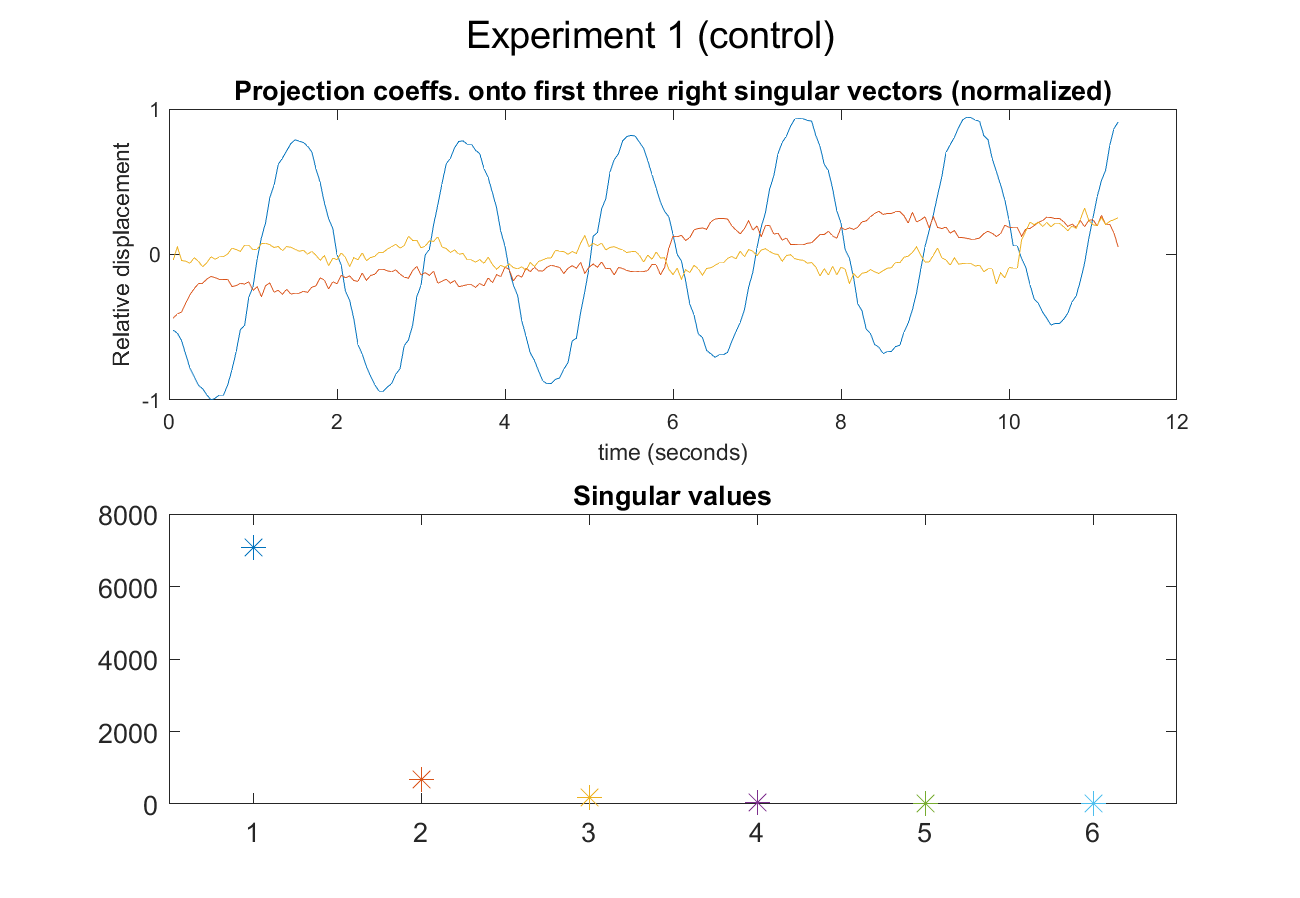
\includegraphics[scale=0.62]{figs/fig1}
\end{figure}
\begin{figure}[!h]
	\centering
	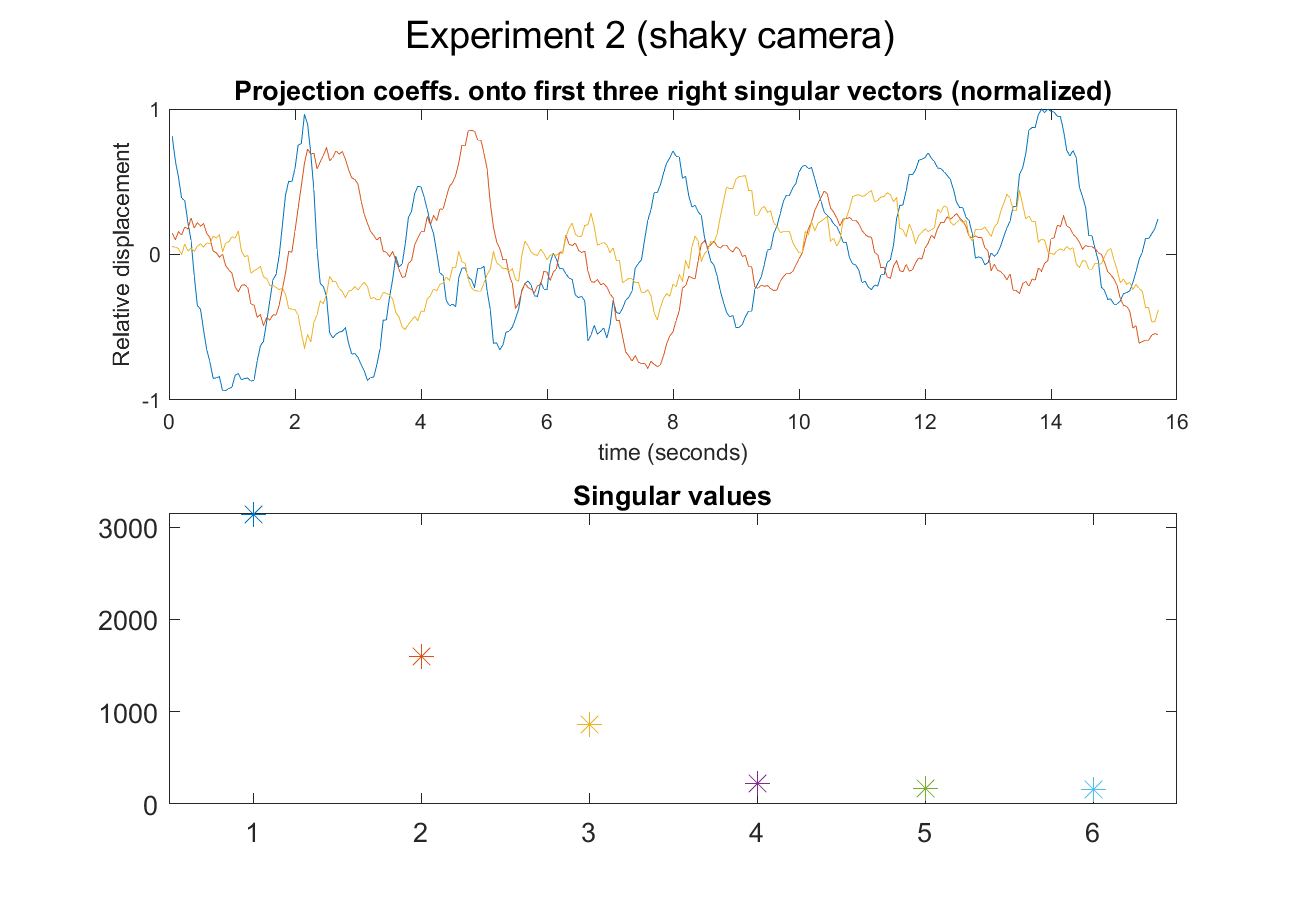
\includegraphics[scale=0.62]{figs/fig2}
	\caption{Results of experiments 1 and 2}
\end{figure}
\begin{figure}[!h]
	\centering
	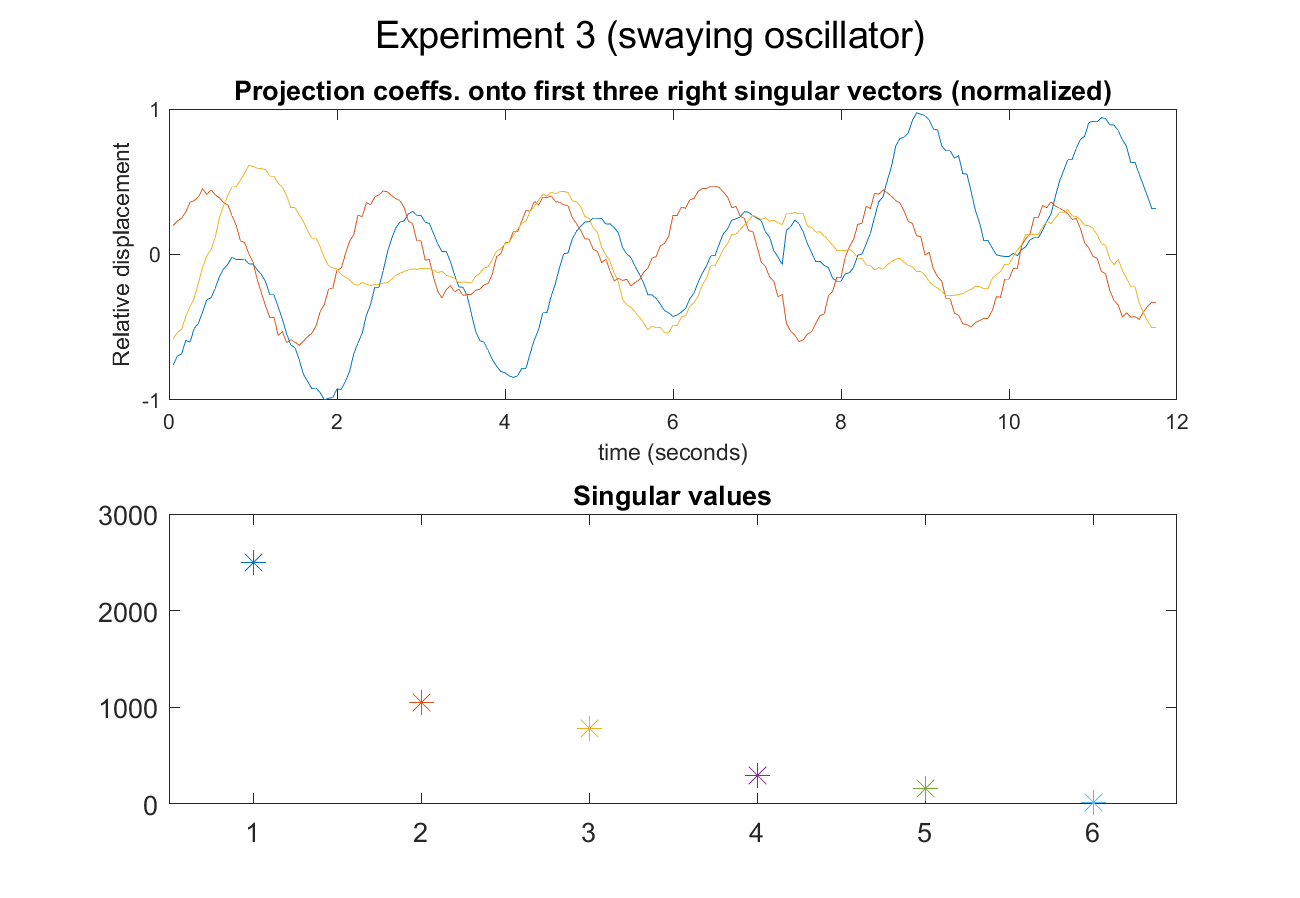
\includegraphics[scale=0.62]{figs/fig3}
\end{figure}
\begin{figure}[!h]
	\centering
	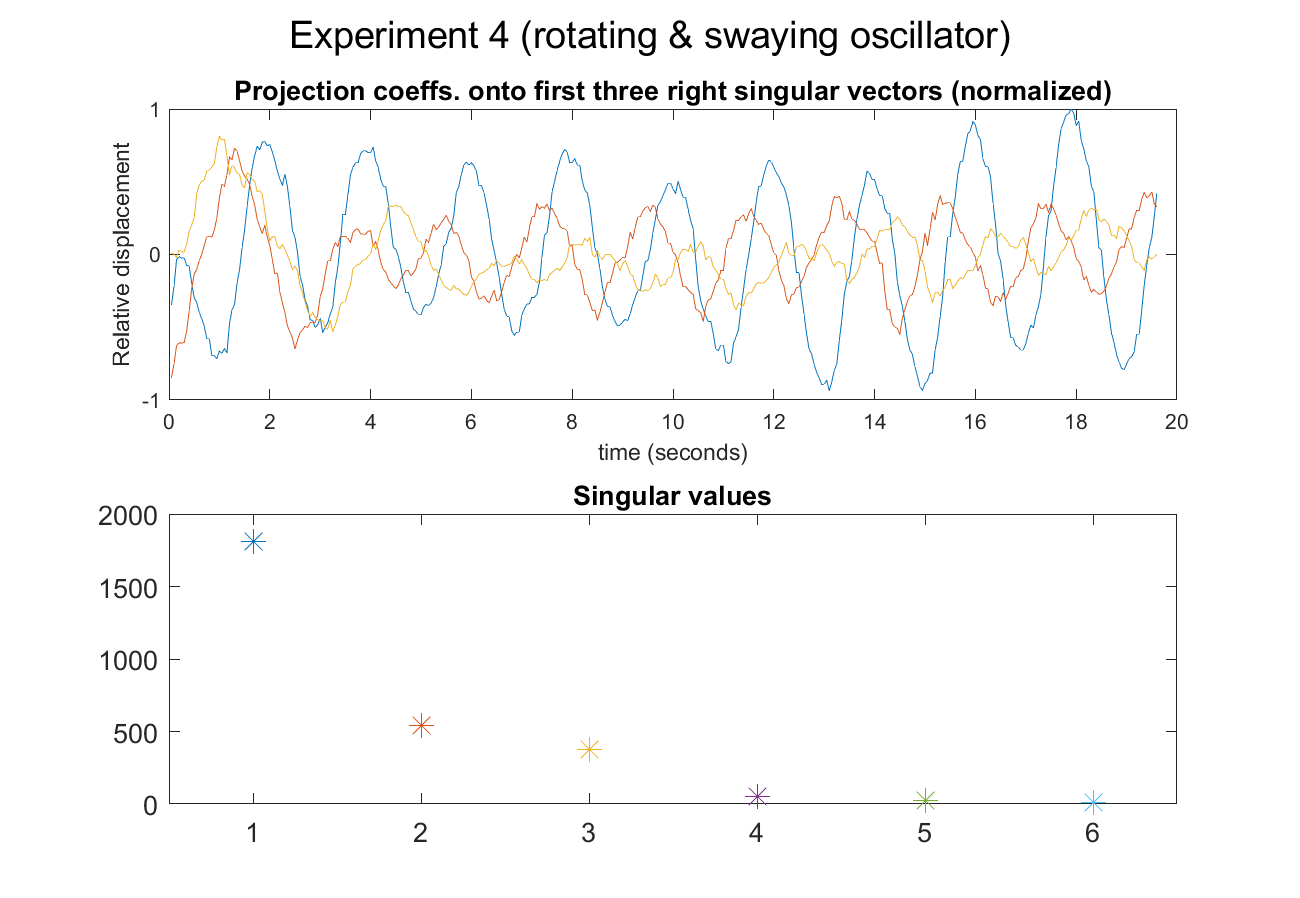
\includegraphics[scale=0.62]{figs/fig4}
	\caption{Results of experiments 3 and 4}
\end{figure}

\newpage 
\;\\\newpage
The first right singular vectors for each of the four experiments are

\begin{equation}
	\begin{bmatrix}
		0.0008\\0.5600 \\
		0.0068 \\
		0.6739 \\
		0.4788\\
		0.0547
	\end{bmatrix}, \begin{bmatrix}
	0.0176 \\ -0.3494 \\ 0.2758 \\ -0.8822 \\ -0.1516 \\ 0.0146
\end{bmatrix}, \begin{bmatrix}
0.0710 \\ 0.4762 \\ 0.2341 \\ 0.8352 \\ 0.0151 \\ -0.1250
\end{bmatrix}, \begin{bmatrix}
-0.03335 \\ 0.4645 \\ -0.0030 \\ 0.8848 \\ 0.0150 \\ -0.0046
\end{bmatrix}
\label{eqn:vector}
\end{equation}

\subsection{Results and interpretation of each experiment}
For all graphs, the result of projecting the data onto the first three right singular vectors has been displayed. The last three singular vectors correspond to very small singular values in each experiment, and the resulting projection would clutter the graph.

Experiment 1 is the control experiment performed under ideal circumstances. The first singular value is much larger than the others, suggesting that the data varies in only one dimension. Though this projection appears sinusoidal, its average displacement seems to wander from the mean of $0$. One possible explanation is that the location-tracking algorithm latched on to a different part of the bucket. With data captured over a longer window, Algorithm~\ref{alg:locate} might capture more reliable data.

Experiment 2 involves shaky cameras. The second and third singular values are more significant than in any other experiment, suggesting that a high degree of variance was captured. The method of PCA identifies the components with the greatest variance, and it is possible that the noise presented too much noise for PCA to deal with. It is also possible that Algorithm~\ref{alg:locate} was unable to perform with so much noise. This experiment is particularly susceptible to experimental error; the initial frames were synchronized manually, and this may have been done improperly since it is difficult to synchronize noisy video data without a clock recorded.

Experiment 3 involves a oscillator with additional sway in the other two dimensions, and these dimensions appear to have been captured well. The second and third singular values are of comparable magnitude, and the projection coefficients appear to form independent sinusoids. This corresponds well with the actual situation of an object oscillating in the vertical dimension with spring-mass behavior, and swaying in the other two horizontal dimensions with pendular behavior.

Experiment 4 is very much like experiment 3 except the mass is also rotating (and the data is captured for a bit longer). Since the angular dynamics in a spring-mass system or a pendulum are virtually independent of translational motion (looking at you, Coriolis force), the oscillation in each dimension should be unaffected. If the location-tracking algorithm is ideal, we should expect similar results to experiment 3, which is fortunately what we see.
\section{Summary and Conclusions}

In all experiments, the first singular value is dominant, the second and third singular values are lesser yet still significant, and the last three singular values are negligible. The question arises, "are the three significant singular values an artifact of using three cameras?" I think the dominant singular vector from experiment 1 in result~\ref{eqn:vector} provides evidence against this question since the SVD was able to identify the main sources of variance occurred in $y_1, y_2, x_3$. This makes sense because cameras 1 and 2 recorded the motion vertically, and camera 3 recorded the motion horizontally.

The orientation of the cameras is the same for all four experiments, yet the dominant singular vectors of experiments do not all capture this. I should expect $y_1,y_2,x_3$ to be dominant in all singular vectors. This is true for those resulting from experiments 1 and 2. In experiment 3, only $y_1$ and $y_2$ seem to dominate the variance, and so the SVD was unable to discern much of use from the third camera. It is possible that the data from the third camera was simply not useful for capturing the mass-spring oscillation. It is also possible that the third camera was particularly susceptible to error arising from Algorithm~\ref{alg:locate}.

The fact that experiment 2 performs so poorly suggests that either Algorithm~\ref{alg:locate} does not deal well with noisy videos, or that the SVD does not deal well with noisy data. Because the SVD is a statistical method--it identifies independent axes of variance--it makes sense that noise manifests as high variance. It is possible that with larger samples, the noise will be averaged out, so further experiments may want to test how well the SVD performs when dealing with a larger sample of noisy data.

% References
\printbibliography
\newpage
% Appendices
\begin{appendices}

% MATLAB Functions
\section{MATLAB Functions}

\begin{itemize}
    \item \texttt{BW = rgbvid2grayvid(RGB)} inputs an RGB video represented as a matrix of dimensions \texttt{height, width, 3, num\_of\_frames} and outputs the result of calling \texttt{rgb2gray} on each frame.
    
    \item \texttt{[U,S,V] = svd(X)} returns the Singular Value Decomposition such that \texttt{U*S*V'=X}
\end{itemize}

% MATLAB Codes
\section{MATLAB Code}

\subsection{main.m}
\inputminted{matlab}{main.m}

\subsection{rgbvid2grayvid.m}
\inputminted{matlab}{rgbvid2grayvid.m}
\end{appendices}

\end{document}